\section{The Proposed Approach}
\label{sec:proposed_approach}
This section presents our proposed method for faulty code prediction with limited data. The model accepts the inputs as assembly instruction sequences obtained by compiling the source files (written in C/C++ programming language). Fig. \ref{fig:c2asm} illustrates an example of a C code and a snippet of its corresponding assembly instructions. The network architecture as shown in Fig. \ref{fig:model} consisting of three main parts (1) a convolutional network, (2) a classifier, and (3) a decoder. Assembled parts of (1)$-$(2) and (1)$-$(3) create two sub-networks to undertake different tasks including classification and an autoencoder for input reconstruction. The rest of this section will describe model details.
\begin{center}
    \begin{figure}
    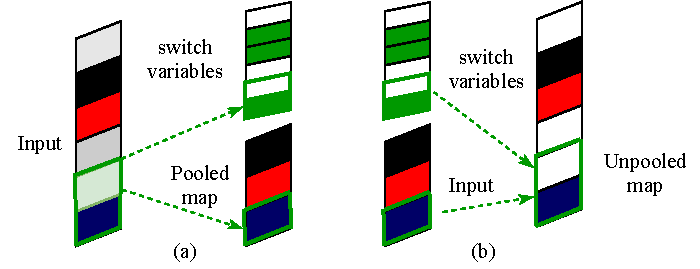
\includegraphics[width=0.6\textwidth]{sections/figures/pool_unpool.pdf}
    \caption{The model architecture. }
    \label{fig:model}
    \end{figure}
\end{center}
\subsection{The convolutional network}
Assembly code is selected as the input of the model. Based on previous studies, assembly instructions are more suitable for software fault prediction than other representations like software metrics and abstract syntax trees (ASTs) \cite{phan2017conv_asm}. Basically, software metrics simply capture surface features of programs, and ASTs just represent the program syntactic structures. While semantic bugs are more relevant to program behaviors than the structures \cite{viet2019transfer}. For this criterion, assembly code should be a selection because assembly instructions are translated into the machine code one by one. To feed into the network, each instruction is encoded as a real-valued vector with thirty dimensions. To learn the vector representations, we collected assembly instruction sequences from all experimental data and trained by the GloVe algorithm \cite{pennington2014glove}.   

\textbf{Vector representation} is the first layer of the networks. After obtaining instruction vectors, we form the lookup table $ E = e_1 \oplus e_2 \oplus ... \oplus e_N \in \mathbb{R}^{N \times d}$, where, $N$ is the number of unique assembly instructions and $d$ is the vector size; $e_i$ is the vector of $i^{th}$ instruction and $\oplus$ is the concatenation operation. Given an input program with instruction sequences $a_1, a_2, ..., a_L$, the embedding matrix is $E_p =  e_{idx(a_1)} \oplus e_{idx(a_2)} \oplus ... \oplus e_{idx(a_L)} \in \mathbb{R}^{L \times d} $,  in which $idx{(a_i)}$ is a mapping function returning the index of the assembly instruction $a_i$ in the lookup table.  
    \begin{center}
        \begin{figure}
        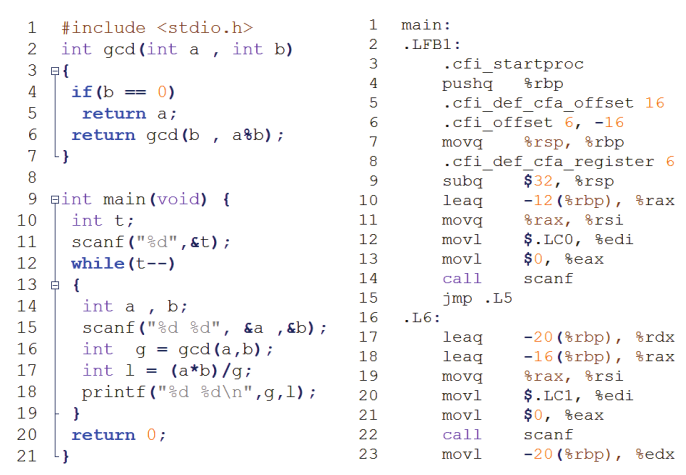
\includegraphics[width=\textwidth]{sections/figures/c2asm.png}
        \caption{A C code example and a snippet of its assembly instructions generated by GCC compiler.}
        \label{fig:c2asm}        
        \end{figure}
    \end{center}
\textbf{Convolutional layers} undertake the most important role in the network. These layers apply a set of filters sliding over sequences to learn local features. Specifically, the filters with sizes of 2 and 3 will capture the relations among 2 and 3 instructions, respectively. Stacking multiple convolutional layers make the network able to learn high-level abstract features and expand the local regions for feature extraction, but more difficult to train. Formally, given a input program with the embedding matrix $E_p =  e^p_1 \oplus e^p_2 \oplus ... \oplus e^p_L \in \mathbb{R}^{L \times d}$, a convolution will transform into a feature map with the same length $C^f =\{c^f_1, c^f_2, ..., c^f_L\}$:
    \begin{equation}
    c_i^f = f(W^f \cdot {e^p}_{i:i+h-1} + b_f)
    \end{equation}
    where $h$ is the filter size,
    $e^p_{i:i+h-1} = e^p_i \oplus e^p_{i+1} \oplus ... \oplus e^p_{i+h-1}$, $W_f \in \mathbb{R}^{h \times d}$, $f$ is an non-linear activation function, and $b_f$ is a bias.
Normally, many filters are used in a convolutional layer to extract features according to different relation aspects. 

\textbf{A pooling layer} is commonly stacked on each convolutional layer to perform dimension reduction. For high dimensional data, downsampling helps to reduce model parameters, and hence to speed up computational time and control overfitting. In the experimental datasets, a program may have up to 3,000 instructions resulting in a $3,000 \time 30$ embedding matrix. In addition, the convolution just transforms the input data without downsampling. Therefore, applying pooling layers is essential.

In pooling layers, each feature map is resized independently. Normally, a pooling layer splits a feature map into non-overlapping regions and then applies the pooling operation for such sub-regions. Two commonly used operations are $max$ and $average$. For example, a max pooling with the filter size of 2 and the stride of 2, the feature map column $C^f$ will be separated into two-value regions, and the greater one of each pair is selected. This results in the pool feature map with size of $L/2$. In the training process, the backward pass simply routes the gradient to the highest value in the forward pass. 

    \begin{center}
        \begin{figure}
        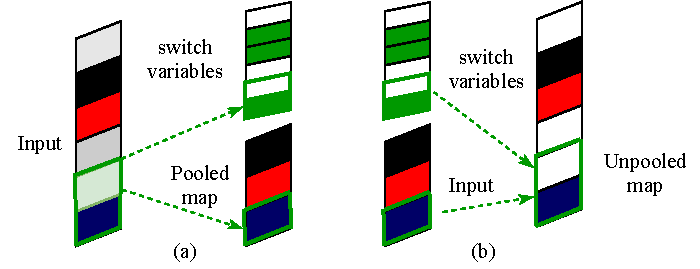
\includegraphics[width=\textwidth]{sections/figures/pool_unpool.pdf}
        \caption{Illustration of pooling (a) and unpooling (b) processes.}
        \label{fig:pool_unpool}        
        \end{figure}
    \end{center}
\subsection{The classifier}
For predicting faulty code, the classifier is built based on the features extracted by the convolutional network. This part includes a global pooling and some fully connected layers.

\textbf{Global pooling}. The last pooling layer in the part (1) is also a high dimensional features. To select the most sophisticated features, a global pooling is applied to pool each feature map into a single value.

\textbf{Fully connected layers} contains neurons that fully connect to all neurons in the previous layer. The activation of the last layer is $softmax$ to convert score values into distribution probabilities.
    \begin{equation}
    \label{eq:softmax}
        \sigma(\textbf{z}_c) = \frac{e^{z_c}}{\sum_{i = 1}^{K}{e^{z_i}}}
    \end{equation}
    where $K$ is the number of target labels, $c = 1, ..., K$, and $\textbf{z} = (z_1, ..., z_K)$

We use categorical cross-entropy to evaluate the classification loss. For an instance $i$, the loss is computed as follows:
    \begin{equation}
    \label{eq:loss_classification}
        L(y_i, \hat{y_i}) = -\sum_{c=1}^{K}{y_{i,c}log(p_{i,c})}
    \end{equation}{}
    where $y_{i,c}$ is the indicator function that has value of 1 if and only if $c$ is the correct target for the instance $i$. $p_{i,c}$ is the predicted probability for the class $c$ as in Equation \ref{eq:softmax}.
\subsection{The autoencoder}
An autoencoder consists of two segments, the encoder and the decoder (parts 1 and 3) that have symmetric structures. The encoder maps input sequences $\textbf{X}$ by function $\phi$ to latent representations $\textbf{F}$. Inversely, the decoder tries to recreate the original sequences $X$ by function $\psi$. The process can be formulated as follows.
    \begin{equation}
    \begin{split}
        &\phi : \textbf{X} \rightarrow \textbf{F} \\
        &\psi : \textbf{F} \rightarrow \textbf{X} \\
        &\phi, \psi = \underset{\phi, \psi}{\operatorname{argmin}}\left \| \textbf{X} - (\phi \circ  \psi)\textbf{X } \right \|^2    
    \end{split}
    \end{equation}

In the model, both the encoder and the decoder are built up from convolutional layers. A slight difference between the two architectures is that the pooling is used for dimension reduction in the encoder, while the decoder applies an upsampling to expand feature maps. 

The objective of training the autoencoder is to minimize the reconstruction errors. The loss function for an instance $x_i$ is as follows.
    \begin{equation}
    \label{eq:loss_reconstruction}
     \begin{split}
         L(x_i, {x_i}') &= \left \| x_i - {x_i}' \right \|^2 \\
                  &= \left \| x_i - \phi(\psi(x_i)) \right \|^2
    \end{split}
    \end{equation}
    where ${x_i}'$ is the reconstruction that has the same shape as $x_i$.
    
\subsection{Loss function}
The two branches shares the first part and are jointly trained. Therefore, the loss function of the whole model is the combination of classification and reconstruction errors. From equations \ref{eq:loss_classification} and \ref{eq:loss_reconstruction}, training process will minimize the following function.  
\begin{equation}
     \begin{split}
         L_i &= L(y_i, \hat{y_i}) + L(x_i, {x_i}') \\
             &= -\sum_{c=1}^{K}{y_{i,c}log(p_{i,c})} + \left \| x - \phi(\psi(x')) \right \|^2
    \end{split}
    \end{equation}